% bonsai-turbo header figure, paper style. 2:1 canvas, renders to 2560x1280.
% Build: infra/modal/texbuild.py, or locally:
%   pdflatex overview.tex && pdftoppm -png -scale-to-x 2560 -scale-to-y 1280 -singlefile overview.pdf overview
\documentclass[border=0pt]{standalone}
\usepackage{tikz}
\usepackage{amsmath}
\usepackage[T1]{fontenc}
\usepackage{lmodern}
\usetikzlibrary{arrows.meta, positioning, calc, patterns}

\definecolor{ink}{HTML}{111111}
\definecolor{gray1}{HTML}{555555}
\definecolor{gray2}{HTML}{999999}
\definecolor{fillg}{HTML}{E8E8E8}
\definecolor{acc}{HTML}{B03A2E}   % muted red, classic paper accent

\begin{document}
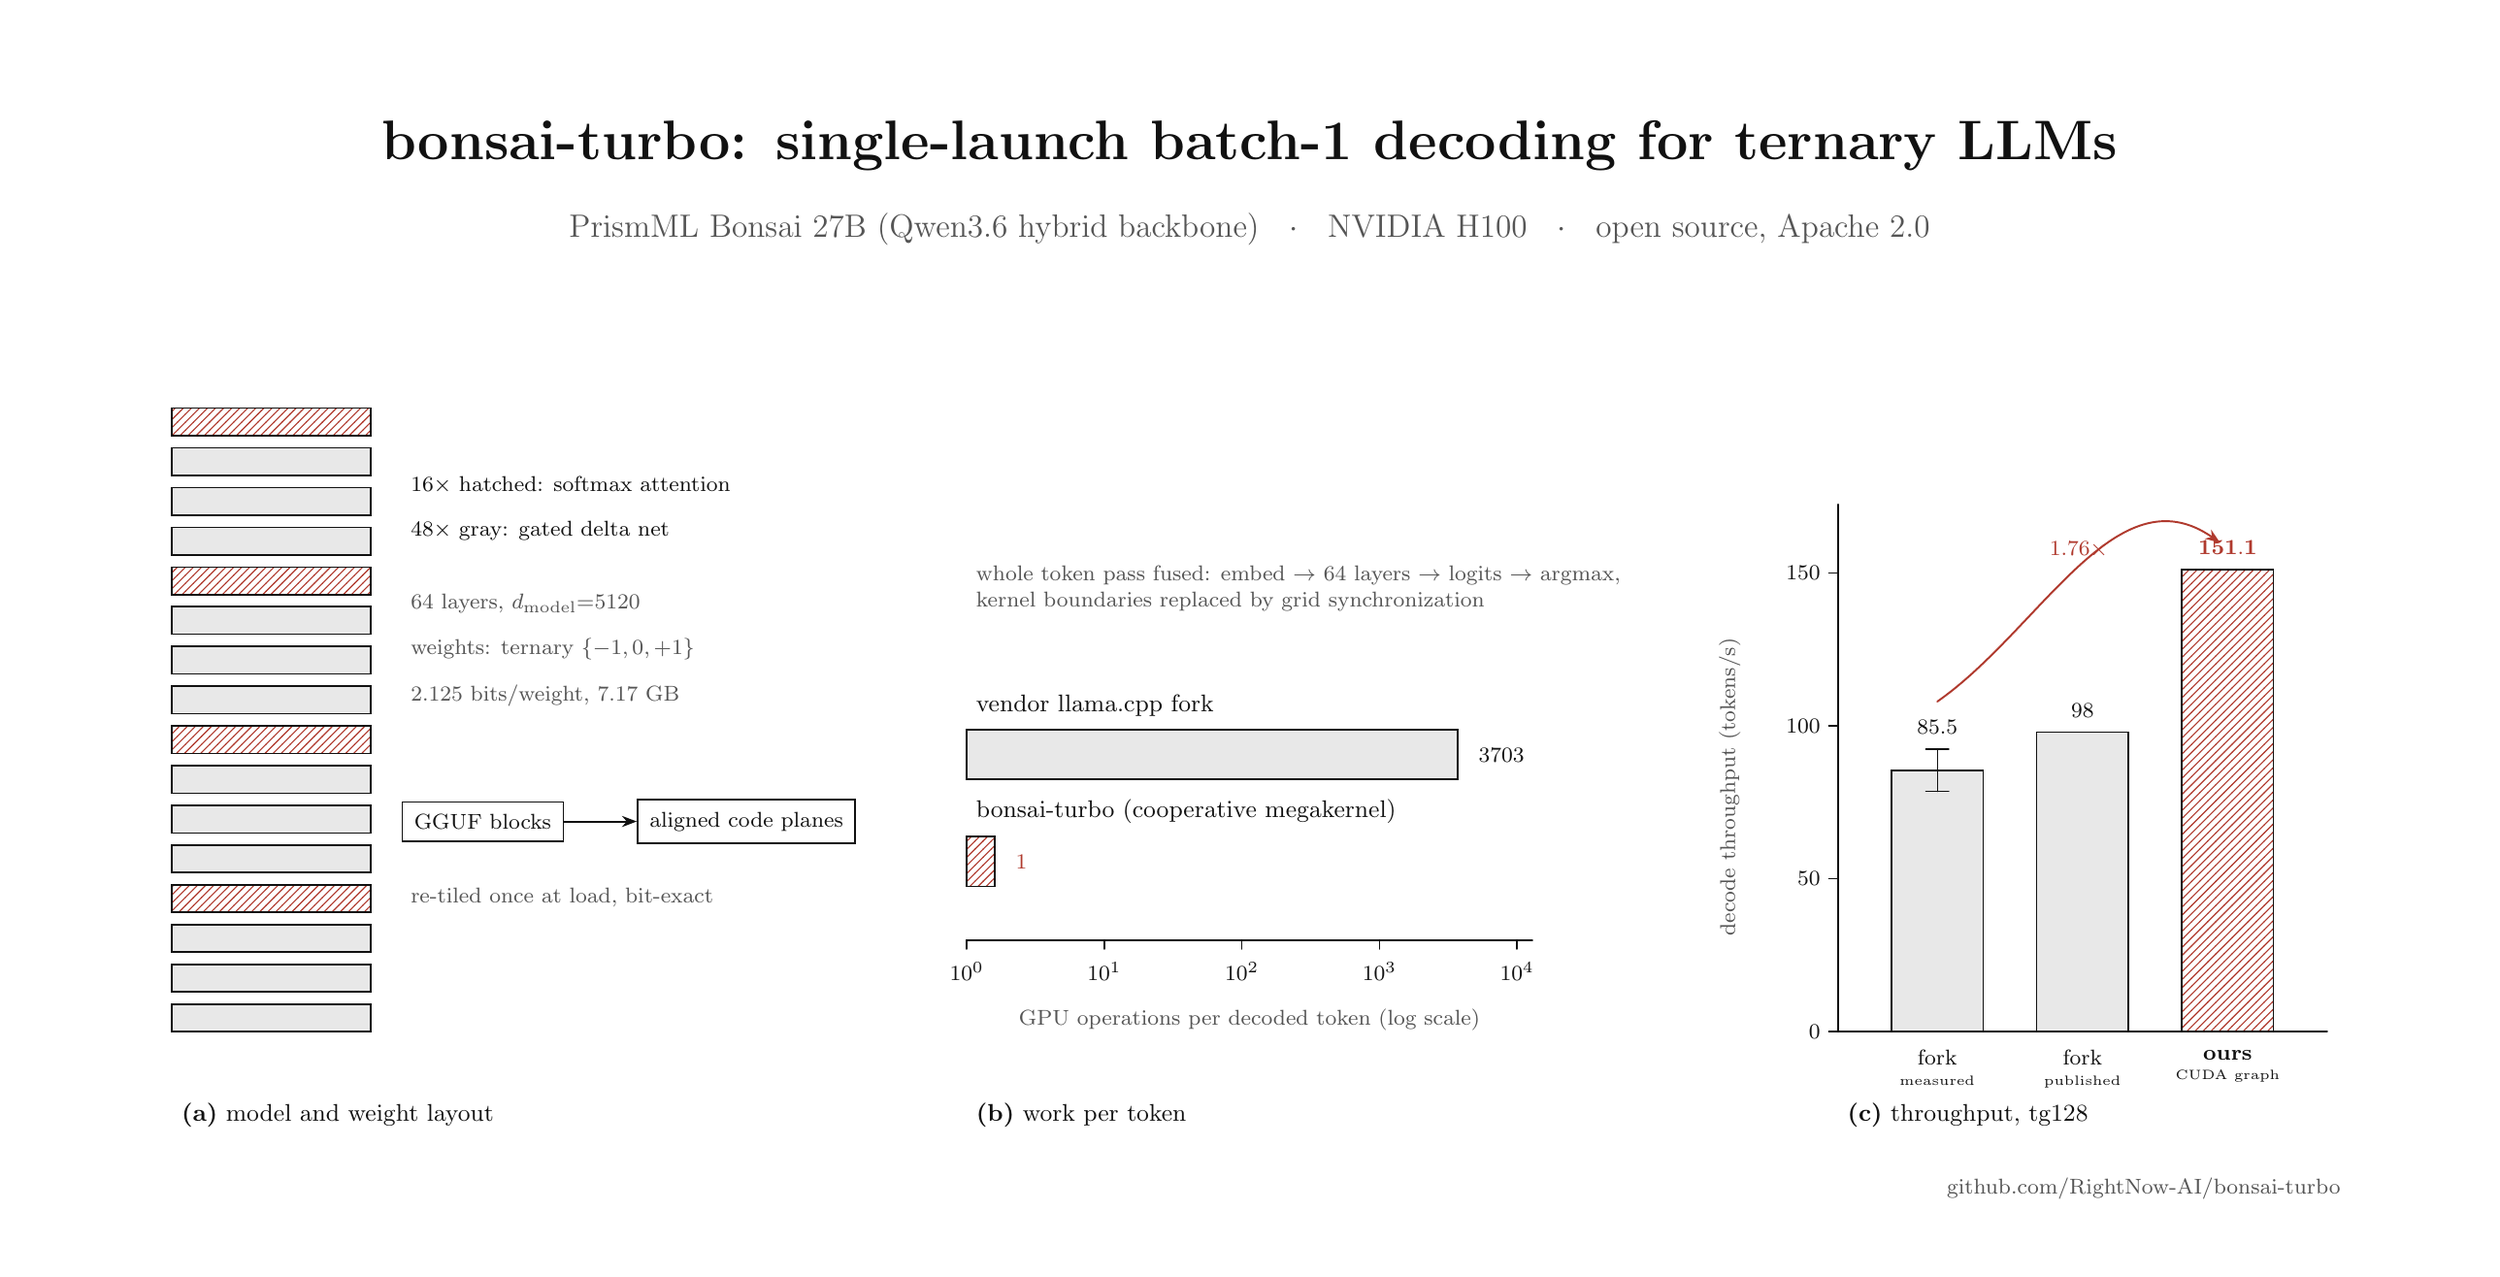
\begin{tikzpicture}[x=1cm, y=1cm, line cap=round,
    every node/.style={text=ink},
    axis/.style={ink, line width=0.7pt},
    tick/.style={ink, line width=0.5pt},
    barsty/.style={draw=ink, line width=0.6pt},
    flow/.style={-{Stealth[length=5.5pt]}, line width=0.7pt, ink}
]

% ---------------- canvas (32 x 16 = 2:1), white ----------------
\fill[white] (0,0) rectangle (32,16);

% ---------------- heading, paper style ----------------
\node[anchor=center, font=\fontsize{21}{24}\selectfont\bfseries] at (16,14.45)
    {\textsc{bonsai-turbo}: single-launch batch-1 decoding for ternary LLMs};
\node[anchor=center, font=\fontsize{11.5}{14}\selectfont, text=gray1] at (16,13.35)
    {PrismML Bonsai 27B (Qwen3.6 hybrid backbone) \; $\cdot$ \; NVIDIA H100 \; $\cdot$ \; open source, Apache 2.0};

% ================= panel (a): model and memory layout =================
\begin{scope}[shift={(1.9,2.85)}]
    % layer stack, thin outlines; every 4th layer hatched = softmax attention
    \foreach \i in {0,...,15} {
        \pgfmathsetmacro{\yy}{\i*0.52}
        \pgfmathparse{int(mod(\i+1,4))}
        \ifnum\pgfmathresult=0
            \draw[barsty, pattern=north east lines, pattern color=acc] (0,\yy) rectangle (2.6,\yy+0.36);
        \else
            \draw[barsty, fill=fillg] (0,\yy) rectangle (2.6,\yy+0.36);
        \fi
    }
    \node[font=\small, anchor=west] at (3.0,7.15) {\footnotesize $16\times$ hatched: softmax attention};
    \node[font=\small, anchor=west] at (3.0,6.55) {\footnotesize $48\times$ gray: gated delta net};
    \node[font=\small, anchor=west, text=gray1] at (3.0,5.6) {\footnotesize 64 layers, $d_{\text{model}}{=}5120$};
    \node[font=\small, anchor=west, text=gray1] at (3.0,5.0) {\footnotesize weights: ternary $\{-1,0,+1\}$};
    \node[font=\small, anchor=west, text=gray1] at (3.0,4.4) {\footnotesize $2.125$ bits/weight, $7.17$ GB};

    % mini flow: gguf -> re-tile -> dp4a planes
    \node[draw=ink, line width=0.6pt, font=\footnotesize, inner sep=4.5pt, anchor=west] (g) at (3.0,2.75) {GGUF blocks};
    \node[draw=ink, line width=0.6pt, font=\footnotesize, inner sep=4.5pt, right=0.95 of g] (r) {aligned code planes};
    \draw[flow] (g) -- (r);
    \node[font=\footnotesize, text=gray1, anchor=west] at (3.0,1.75) {re-tiled once at load, bit-exact};

    \node[font=\small, anchor=west] at (0,-1.1) {\textbf{(a)} model and weight layout};
\end{scope}

% ================= panel (b): work per decoded token =================
\begin{scope}[shift={(12.3,4.05)}]
    % log-scale horizontal axis: 10^0 .. 10^4 over 7.2cm
    \newcommand{\lx}[1]{(ln(#1)/ln(10))*1.8}
    \draw[axis] (0,0) -- (7.4,0);
    \foreach \e in {0,1,2,3,4} {
        \draw[tick] ({\e*1.8},0) -- ({\e*1.8},-0.12);
        \node[font=\footnotesize, below=2pt] at ({\e*1.8},-0.1) {$10^{\e}$};
    }
    \node[font=\footnotesize, text=gray1] at (3.7,-1.05) {GPU operations per decoded token (log scale)};

    % vendor bar
    \draw[barsty, fill=fillg] (0,2.1) rectangle ({\lx{3703}},2.75);
    \node[font=\footnotesize, anchor=west] at ({\lx{3703}+0.15},2.42) {$3703$};
    \node[font=\small, anchor=south west] at (0,2.8) {vendor llama.cpp fork};

    % ours bar
    \draw[barsty, pattern=north east lines, pattern color=acc] (0,0.7) rectangle ({\lx{1.6}},1.35);
    \node[font=\footnotesize, anchor=west, text=acc] at ({\lx{1.6}+0.15},1.02) {$1$};
    \node[font=\small, anchor=south west] at (0,1.4) {bonsai-turbo (cooperative megakernel)};

    \node[font=\footnotesize, text=gray1, anchor=west, align=left] at (0,4.6)
        {whole token pass fused: embed $\rightarrow$ 64 layers $\rightarrow$ logits $\rightarrow$ argmax,\\
         kernel boundaries replaced by grid synchronization};

    \node[font=\small, anchor=west] at (0,-2.3) {\textbf{(b)} work per token};
\end{scope}

% ================= panel (c): measured throughput =================
\begin{scope}[shift={(23.7,2.85)}]
    % y axis, 0..160 tok/s over 6.4cm
    \newcommand{\ty}[1]{(#1)*0.04}
    \draw[axis] (0,0) -- (0,6.9);
    \draw[axis] (0,0) -- (6.4,0);
    \foreach \v in {0,50,100,150} {
        \draw[tick] (0,{\ty{\v}}) -- (-0.12,{\ty{\v}});
        \node[font=\footnotesize, left=3pt] at (0,{\ty{\v}}) {$\v$};
    }
    \node[font=\footnotesize, text=gray1, rotate=90, anchor=south] at (-1.15,3.2) {decode throughput (tokens/s)};

    % bars: fork 85.5 +/- 6.9, published 98, ours 151.1
    \draw[barsty, fill=fillg] (0.7,0) rectangle (1.9,{\ty{85.5}});
    \draw[tick] (1.3,{\ty{78.6}}) -- (1.3,{\ty{92.4}});
    \draw[tick] (1.15,{\ty{78.6}}) -- (1.45,{\ty{78.6}});
    \draw[tick] (1.15,{\ty{92.4}}) -- (1.45,{\ty{92.4}});
    \node[font=\footnotesize, below=2pt, align=center] at (1.3,-0.05) {fork\\[-2pt]{\tiny measured}};

    \draw[barsty, fill=fillg] (2.6,0) rectangle (3.8,{\ty{98}});
    \node[font=\footnotesize, below=2pt, align=center] at (3.2,-0.05) {fork\\[-2pt]{\tiny published}};

    \draw[barsty, pattern=north east lines, pattern color=acc] (4.5,0) rectangle (5.7,{\ty{151.1}});
    \node[font=\footnotesize, above=2pt, text=acc] at (5.1,{\ty{151.1}}) {$\mathbf{151.1}$};
    \node[font=\footnotesize, below=2pt, align=center] at (5.1,-0.05) {\textbf{ours}\\[-2pt]{\tiny CUDA graph}};

    \node[font=\footnotesize, above=2pt] at (1.3,{\ty{92.4}}) {$85.5$};
    \node[font=\footnotesize, above=2pt] at (3.2,{\ty{98}}) {$98$};

    % speedup annotation
    \draw[flow, acc] (1.3,{\ty{108}}) to[out=35, in=145] node[above, font=\footnotesize, text=acc] {$1.76\times$} (5.0,{\ty{160}});

    \node[font=\small, anchor=west] at (0,-1.1) {\textbf{(c)} throughput, tg128};
\end{scope}

% ---------------- repo link ----------------
\node[anchor=east, font=\footnotesize, text=gray1] at (30.4,0.8) {github.com/RightNow-AI/bonsai-turbo};

\end{tikzpicture}
\end{document}
